\subsection{Design og struktur}
Kasseapparatet er designet med MVVM~\cite{MVVM}, med stor fokus på adskilelse af Forretningslag og Præsentationslaget. Dette er sikret ved brug af klasser der står for at styre logikken i grænsefladen samt kommunikere ned i de nedre lag, disse kaldet viewmodels. Disse bliver forklaret nærmere længere nede i kapitel ?.
Vores system er herunder beskrevet ved følgende pakkediagram.	

\begin{figure}[H]
	\centering
	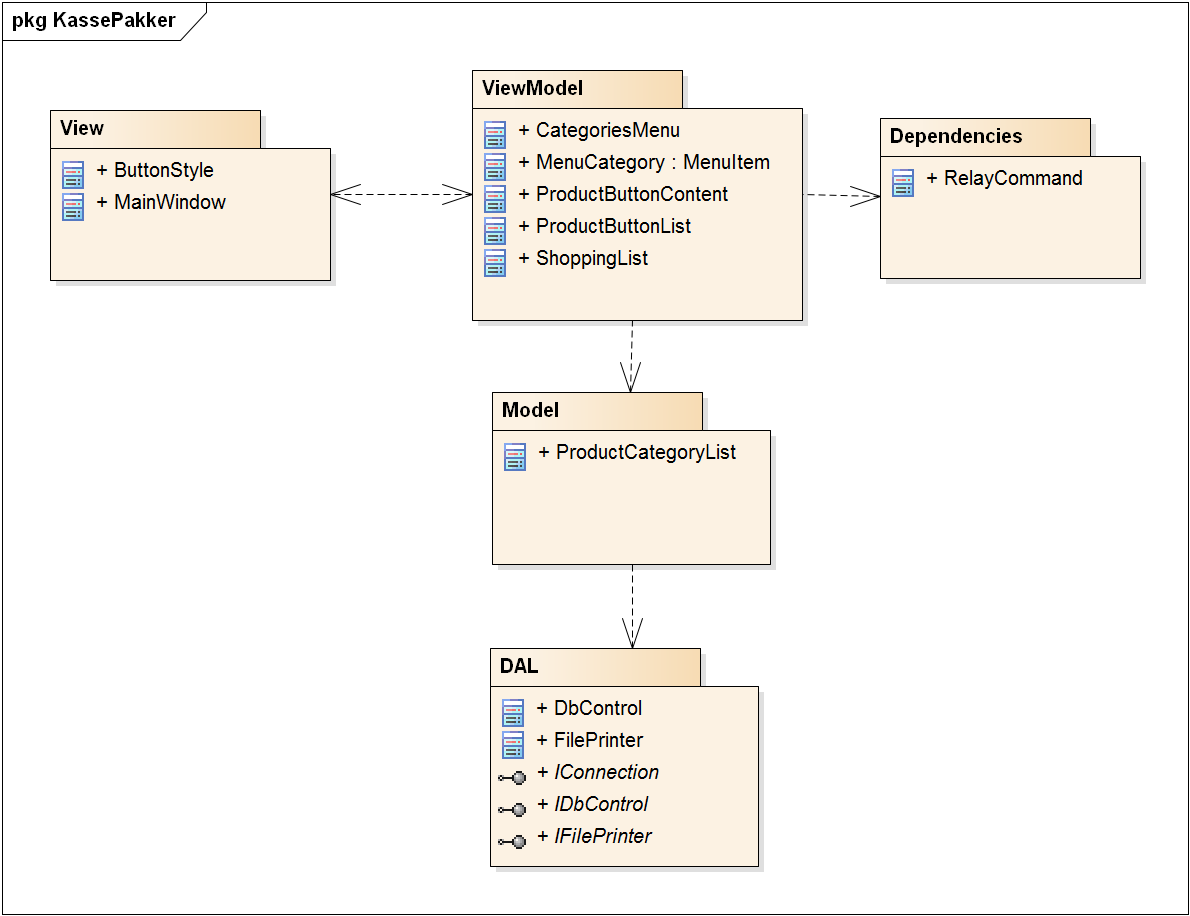
\includegraphics[width=0.8\textwidth]{Systemdesign/Frontend/pics/KassePakker}
	\caption{Pakkediagram over kasseapparat.}
	\label{fig:EndeligeGUI}
\end{figure}

Som man kan se på det ovenstående pakkediagram består kasseapparatet primært af grænsefladen og et data access lag. Dette er fordi at kasse apparatet ikke har som ansvar at kunne oprette/ redigere og slette produkter, men bare at afspejle produkterne i databasen. 

\begin{itemize}
	\item \textbf{View} Views indeholder vores præsentationslagslogik. Det er skrevet i XML og er direkte med til at style vores grænseflade.
	\item \textbf{ViewModel} Er en mediator mellem modellaget og grænsefladen. Viewmodels sikrer at kasseapparatets grænseflade afspejler ændringer der sker nede i systemet, samt kommunikerer grænsefladens ændringer til de lavere lag.
	\item \textbf{Dependencies} Indeholder sourcekode der gør det nemmere at arbejde med commands.
	\item \textbf{Model} Indeholder business logic. Dette er der ikke særligt meget af, da det meste business logic er styret fra administrationssystemet.
	\item \textbf{DAL} Indeholder logik til at kommunikere med CentralServeren og derved Databasen.
\end{itemize}


\subsubsection{Design af elementer}
Herunder vil designet af en stor del af kommunikationen i \gls{KA}tet blive beskrevet, både med klassediagrammer og sekvensdiagrammer.\\

\textbf{Klassediagrammer}\\

\begin{figure}[H]
	\centering
	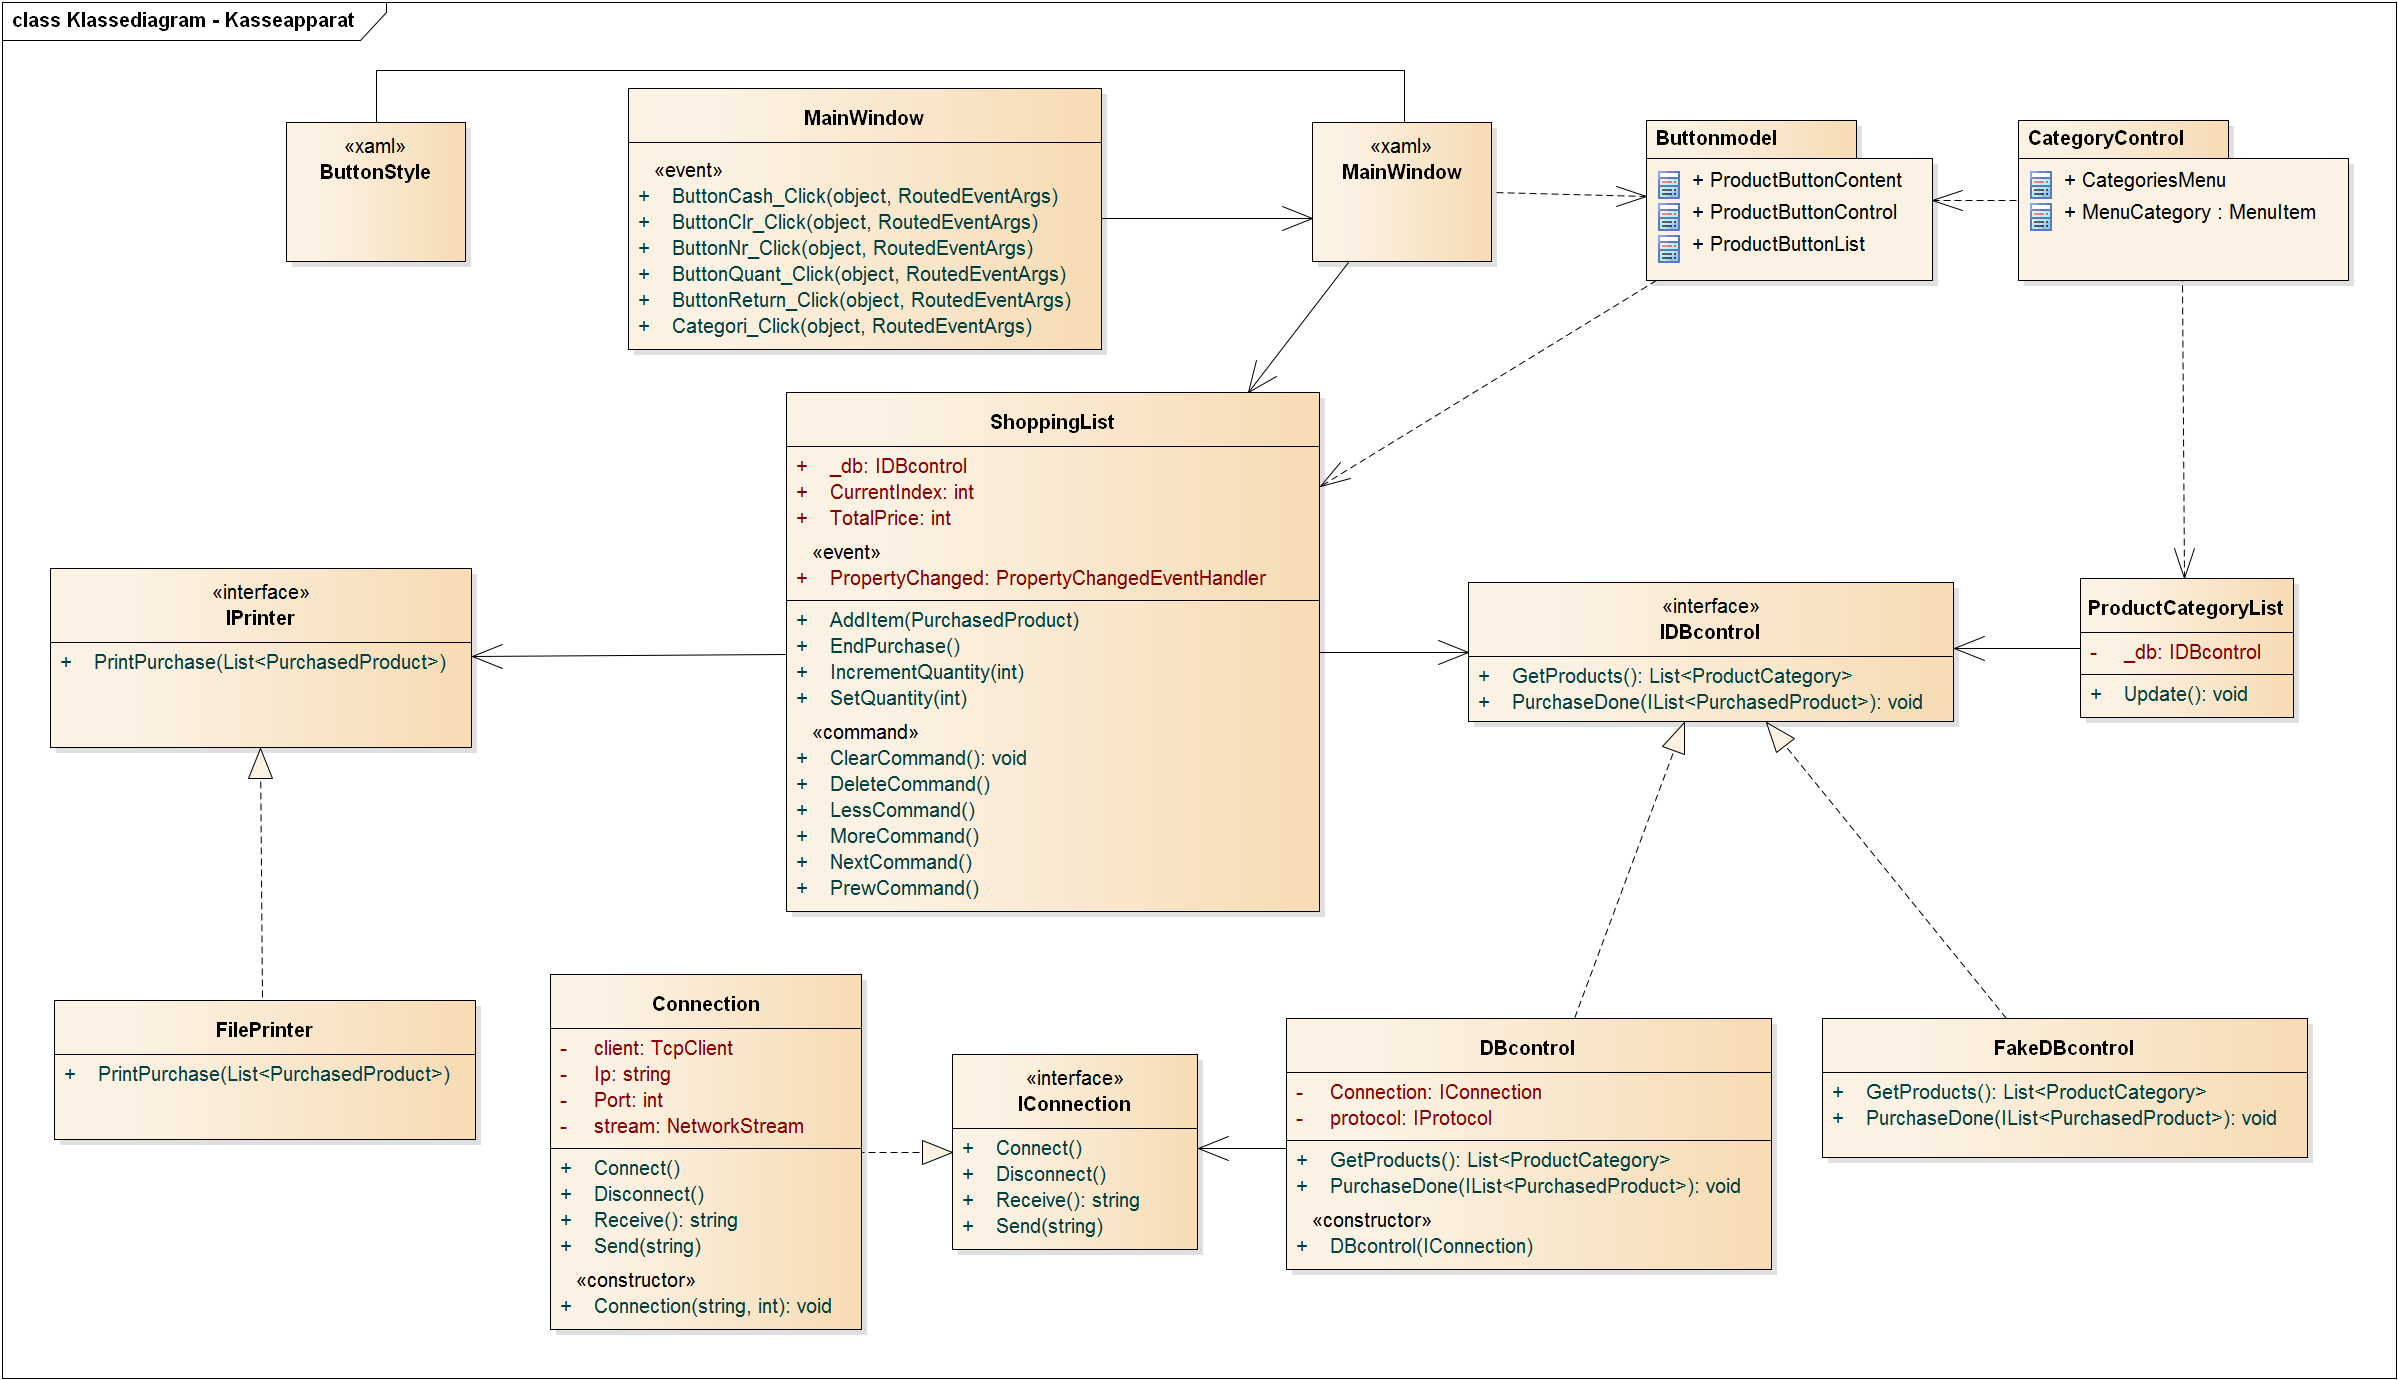
\includegraphics[width=1.2\textwidth, angle=90]{Systemdesign/Frontend/GUI/DesignOgStruktur/Pics/KlassediagramKasseApparat}
	\caption{Klassediagram over kasseapparat.}
	\label{fig:KasseKlasse}
\end{figure}

På figur \ref{fig:KasseKlasse} kan man se hele kasseapparatets software vist ved dens klasser og funktioner. Dog er ViewModels delt op i 2 pakker, hhv. ButtonModel og CategoryControl. Dette er bestemt, da det ville give mere mening at gøre det på denne måde, når man skulle forklare klasserne og deres indbyrdes forhold. Disse forhold vil blive nærmere beskrevet ved figur \ref{fig:ButtonModel} og \ref{fig:CategoryControl} \\
Klassediagrammet er delt op i 3 lag, der skal symbolisere henholdsvis Presentation-, Business Logic- og Data Access Layer. Den øverste række af klasser, repræsenteret ved MainWindow, er presentationlayer. Den midterste række er business logic, repræsenteret ved ShoppingList. Den nederste række er data access layer, repræsenteret ved Connection.

\begin{figure}[H]
	\centering
	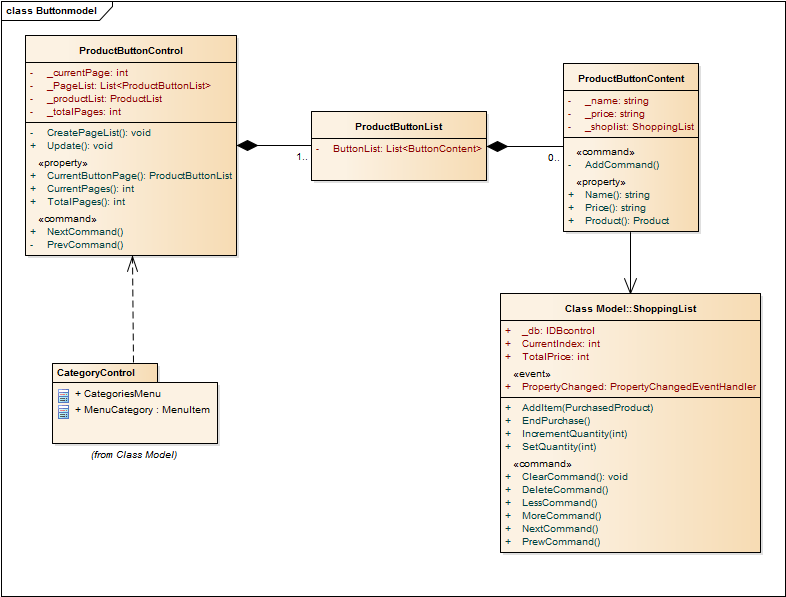
\includegraphics[width=0.7\textwidth]{Systemdesign/Frontend/GUI/DesignOgStruktur/Pics/KlassediagramButtonModel}
	\caption{Klassediagram over ViewModel pakken ButtonModel.}
	\label{fig:ButtonModel}
\end{figure}

På figur \ref{fig:ButtonModel} ser man ViewModel pakken buttonmodel, der står for produktknapperne i grænsefladen. Disse objekter sikrer at man kan skifte produktside og ved tryk på en knap kan et produkt tilføjes til shoppinglist som er indkøbskurven på \gls{KA}tet. For at opsætte denne pakke blev der først opsat et sekvensdiagram set på figur \ref{fig:SekvensUpdatePCL}. Sekvensdiagrammet viser hvordan knapperne bliver oprettet.

\begin{figure}[H]
	\centering
	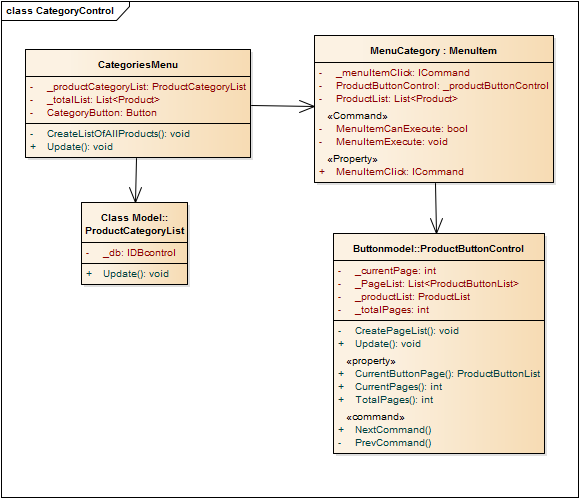
\includegraphics[width=0.7\textwidth]{Systemdesign/Frontend/GUI/DesignOgStruktur/Pics/KlassediagramCategoryControl}
	\caption{Pakkediagram over ViewModel pakken CategoryControl.}
	\label{fig:CategoryControl}
\end{figure}

CategoryControl er en ViewModel der står for at kontrollere produktkategori valg og dermed hvilke produkter der vises i grænsefladen. Denne ViewModel kender til ProductButtonControl, da den derved kan oprette de ønskede produktknapper ved tryk på en kategori. Viden om eksisterende kategorier får pakken ved ProductCategoryList. \\

\textbf{Sekvensdiagrammer} \\
For at forstå kommunikationen mellem de forskellige klasser/pakker er de følgende sekvensdiagrammer blevet opsat. \\

\begin{figure}[H]
	\centering
	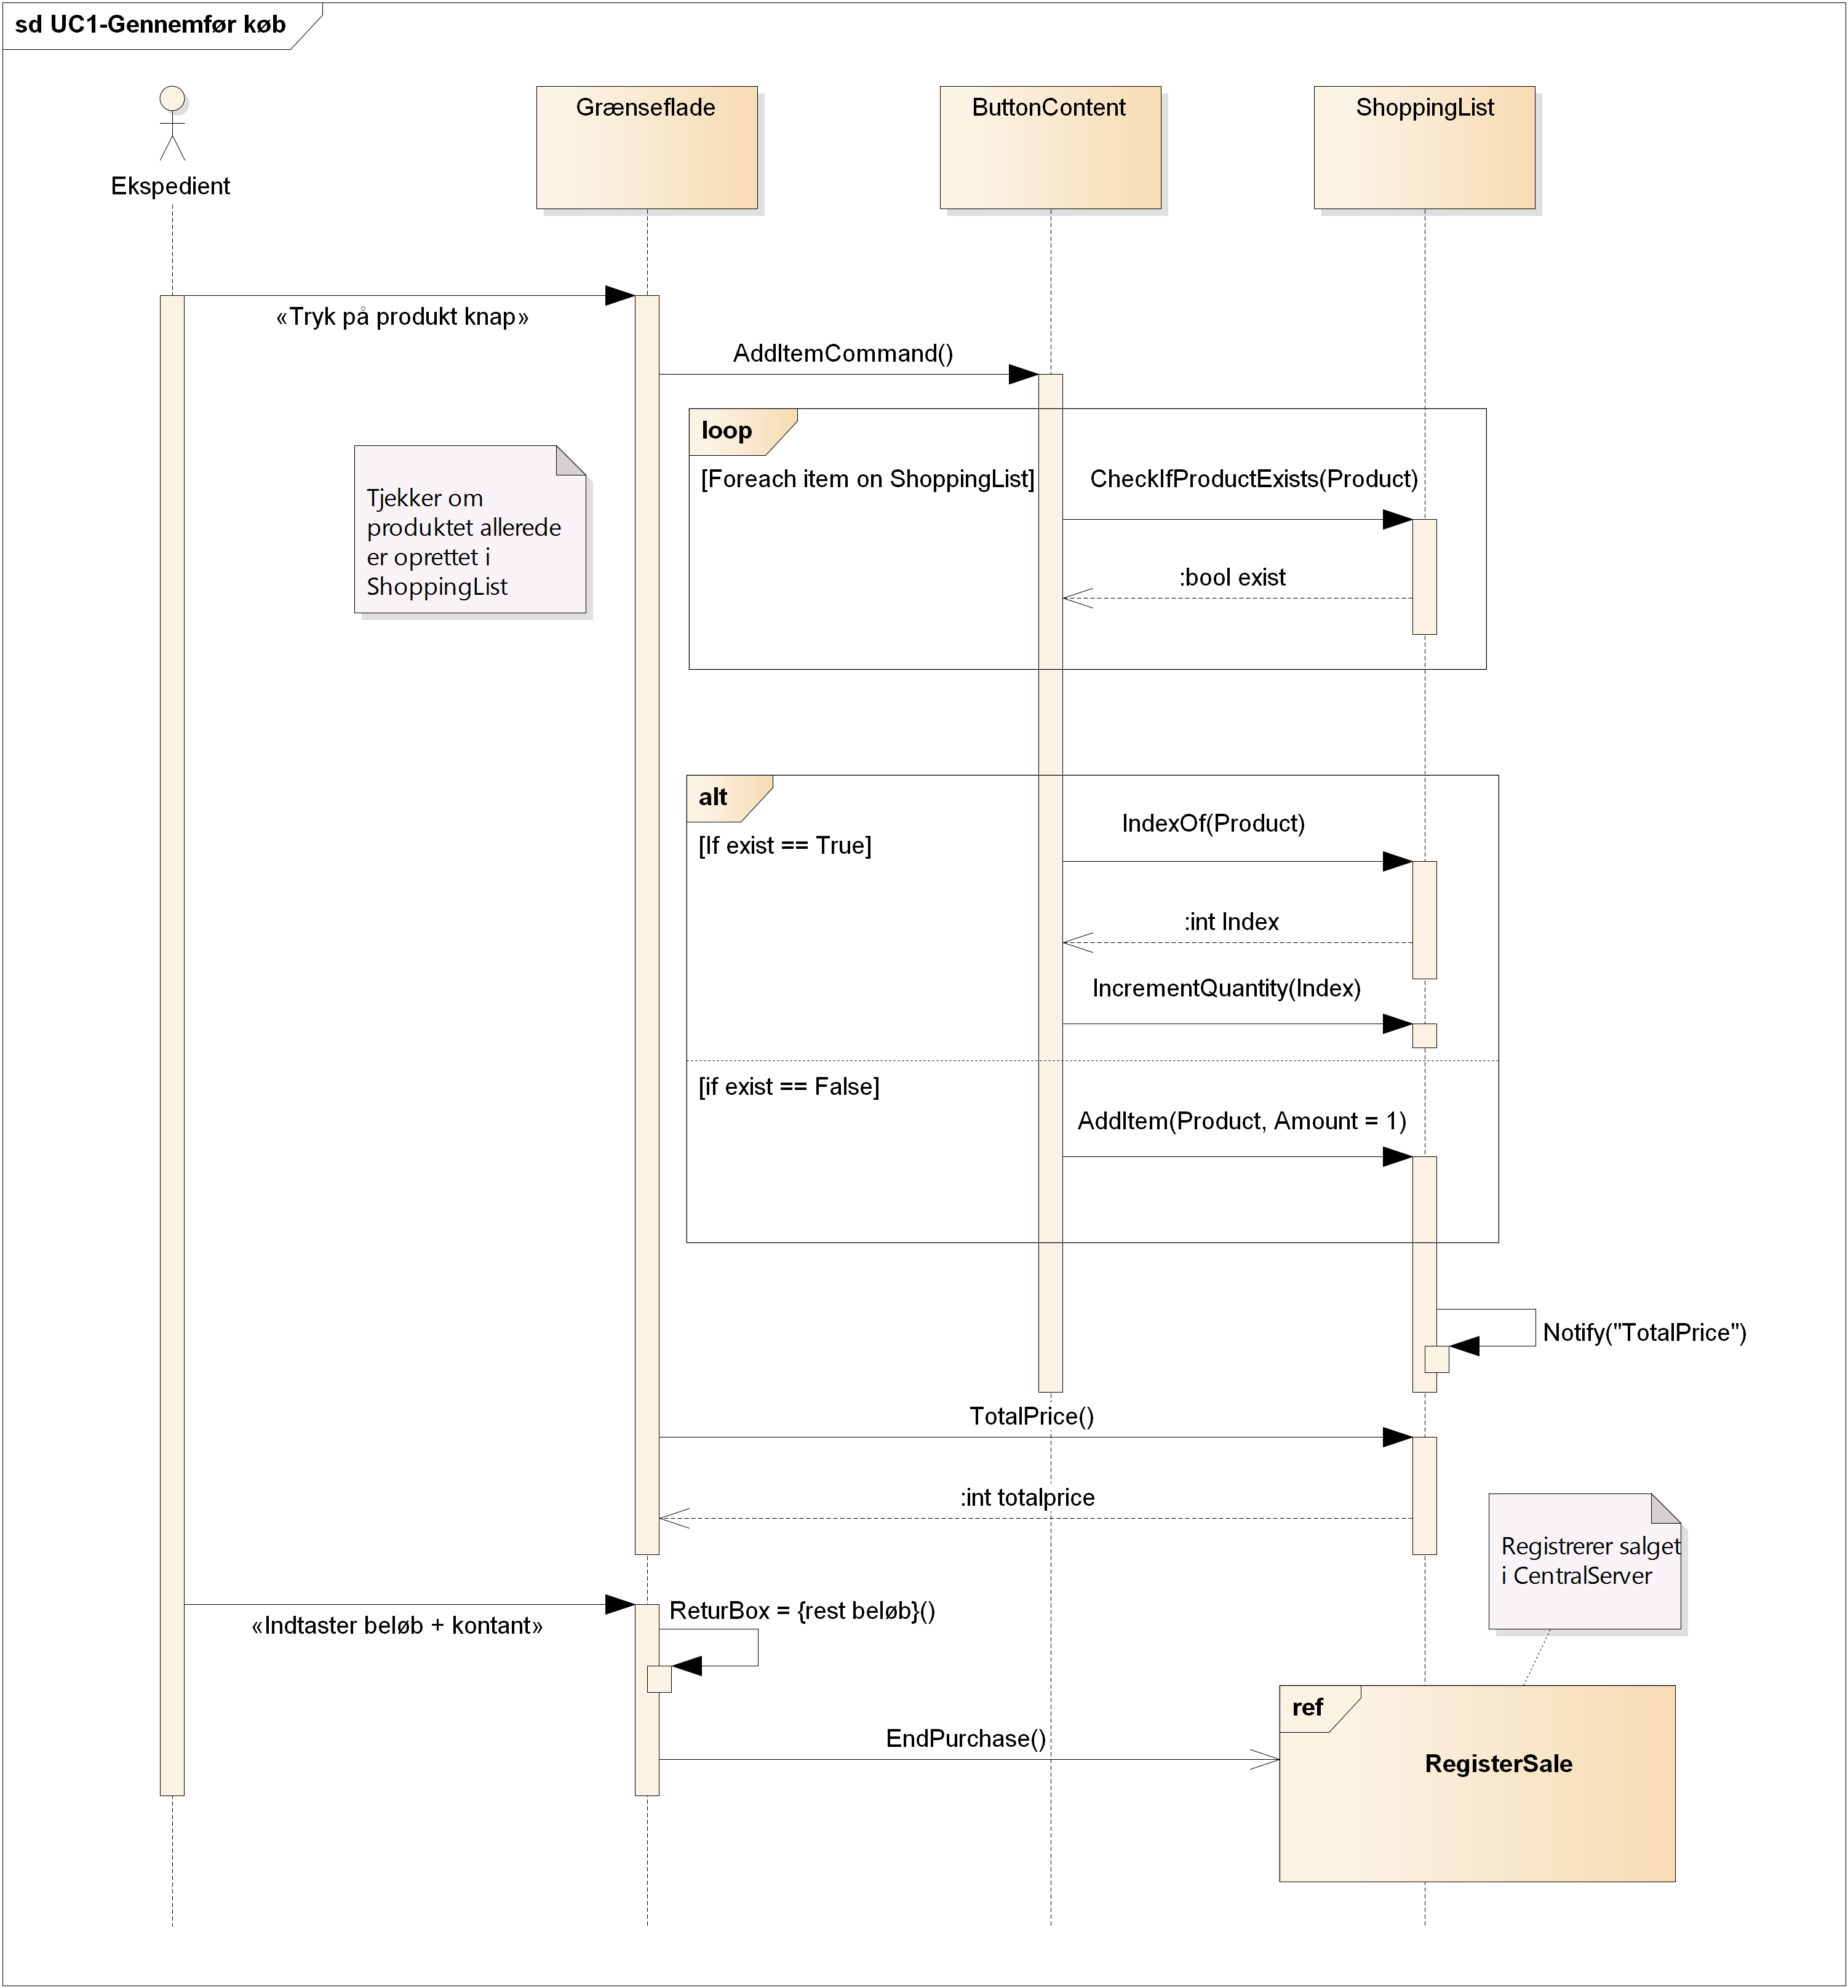
\includegraphics[width=1\textwidth]{Systemdesign/Frontend/GUI/Pics/Sekvensdiagram-TilfoejProdukt2}
	\caption{Sekvensdiagram over tilføjelse af produkt til shoppinglist}
	\label{fig:SekvensUC1}
\end{figure}

På figur \ref{fig:SekvensUC1} er der opsat et sekvensdiagram over Use Case 1 - Gennemfør køb. Her kan man se hvad der sker når en ekspedient starter et salg ved at vælge et produkt i grænsefladen. Når knappen bliver trykket ned, så kalder viewet AddItemCommand i ViewModellen ButtonContent. Dette command tjekker så om der allerede er tilføjet et produkt i shoppinglist. Hvis der er, inkrementeres produktet. Hvis ikke så tilføjes det. Herefter notifier shoppinglist på at der er ændret på totalprice og den nye værdi hentes derefter af viewet. \\
Nu da produktet er tilføjet til shoppinglist kan ekspedienten tage imod penge fra kunden, trykke beløbet ind og så til sidst trykke på kontant. Herefter bliver der kaldt EndPurchase over i shoppinglist. Resten af sekvensen er vist ved sekvensdiagrammet på figur \ref{fig:SekvensRegisterSale}. Dette diagram er lagt for sig selv for at gøre det ovenstående sekvensdiagram mere overskueligt. Det første sekvensdiagram viser indtastning af produkter og det næste viser registrering af salg.

\begin{figure}[H]
	\centering
	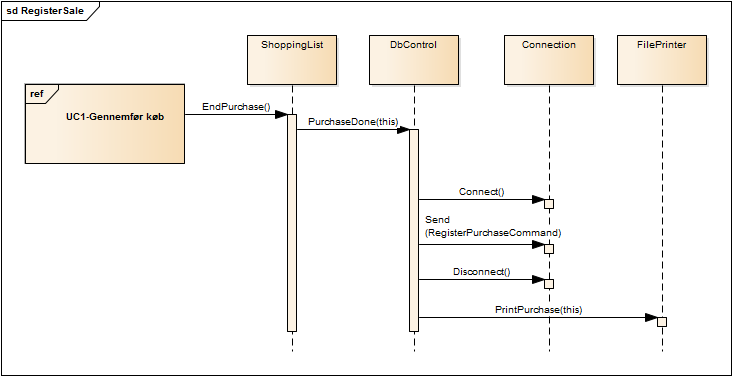
\includegraphics[width=1\textwidth]{Systemdesign/Frontend/GUI/DesignOgStruktur/Pics/RegisterSale}
	\caption{Sekvensdiagram over registrering af salg.}
	\label{fig:SekvensRegisterSale}
\end{figure}

Sekvensdiagrammet på figur \ref{fig:SekvensRegisterSale} viser registrering af salg ved færdigt salg. Først kaldes ShoppingList med EndPurchase. Denne kaldes så DbControl med en reference til sig selv. Dette betyder at DbControl får adgang til alle de produkter som er tilføjet. Herefter kalder DbControl \textit{connect} for at forbinde til \gls{CS}. Herefter sender DbControl en \textit{RegisterPurchaseCommand} som fortæller CentralServer at der er gennemført en handel, og samtidig hvilke produkter der er solgt. Dette betyder at \gls{CS} kan producere en rekvisitionskvittering. Til sidst disconnecter DbControl forbindelsen til \gls{CS} ved et kald til \textit{disconnect} i Connection og kalder derefter PrintPurchase i FilePrinter som derved producerer en salgskvittering.

\begin{figure}[H]
	\centering
	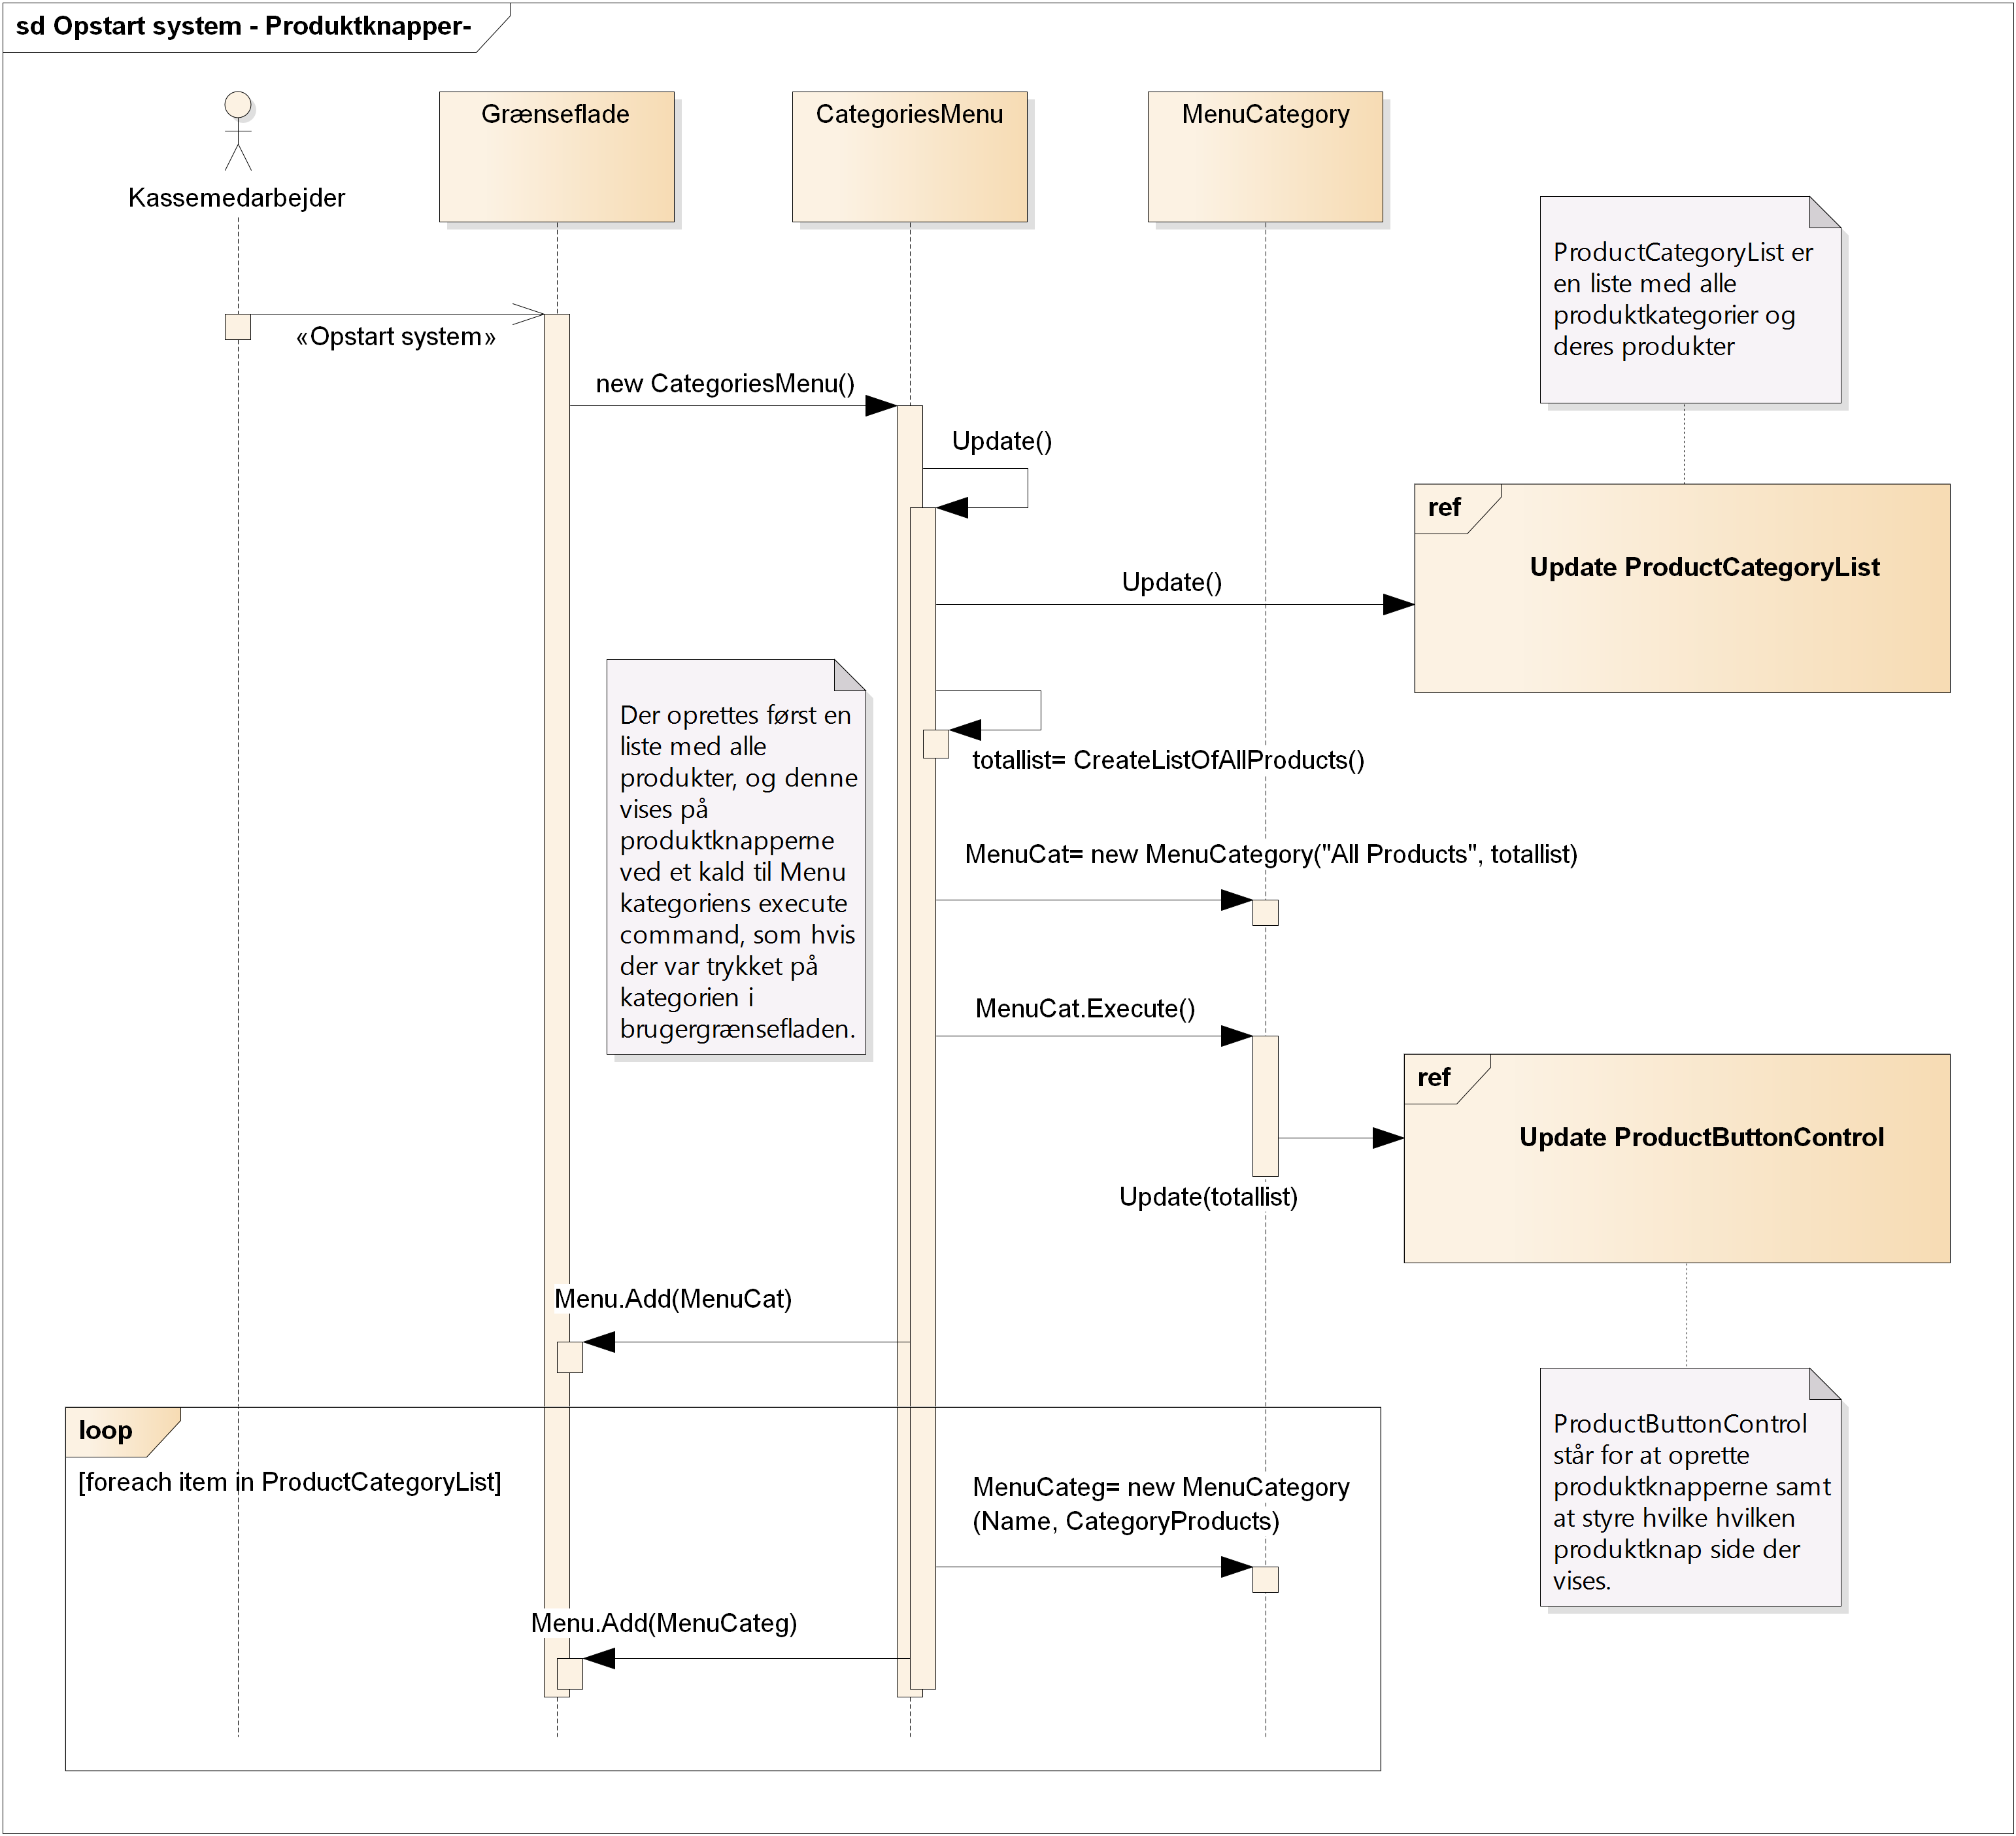
\includegraphics[width=1\textwidth]{Systemdesign/Frontend/GUI/DesignOgStruktur/Pics/OpstartSystem2}
	\caption{Sekvensdiagram over opstart system}
	\label{fig:SekvensOpstart}
\end{figure}

Sekvensdiagrammet på figur \ref{fig:SekvensOpstart} viser hvad der sker når programmet påbegyndes i forhold til oprettelse af produktknapper samt kategori knappen. Først oprettes CategoriesMenu som i sin konstruktor kalder metoden Update. Denne metode kalder så update på ProductCategoryList\footnote{Se figur \ref{fig:SekvensUpdatePCL} samt tilhørende forklaring}. Dernæst oprettes listen totalList, som indeholder alle produkter uanset kategori. Denne liste bliver brugt ved oprettelsen af den første MenuCategory hvilket gør så den første kategori er en kategori med alle produkter. \\
For at sikre at der er produkter vist i produktknapperne ved opstart kaldes MenuCategoriens command Execute, der opdaterer ProductButtonControl med dens tilknyttede produktliste, her totalList \footnote{Se figur \ref{fig:SekvensUpdatePBC} samt tilhørende forklaring}. Nu tilføjes MenuCategorien til ContextMenuen, som er en menu der er tilknyttet en menuknappen i grænsefladen. Derefter oprettes der en MenuCategory for hver eksisterende kategori, og hver af disse tilføjes i ContextMenuen.

\begin{figure}[H]
	\centering
	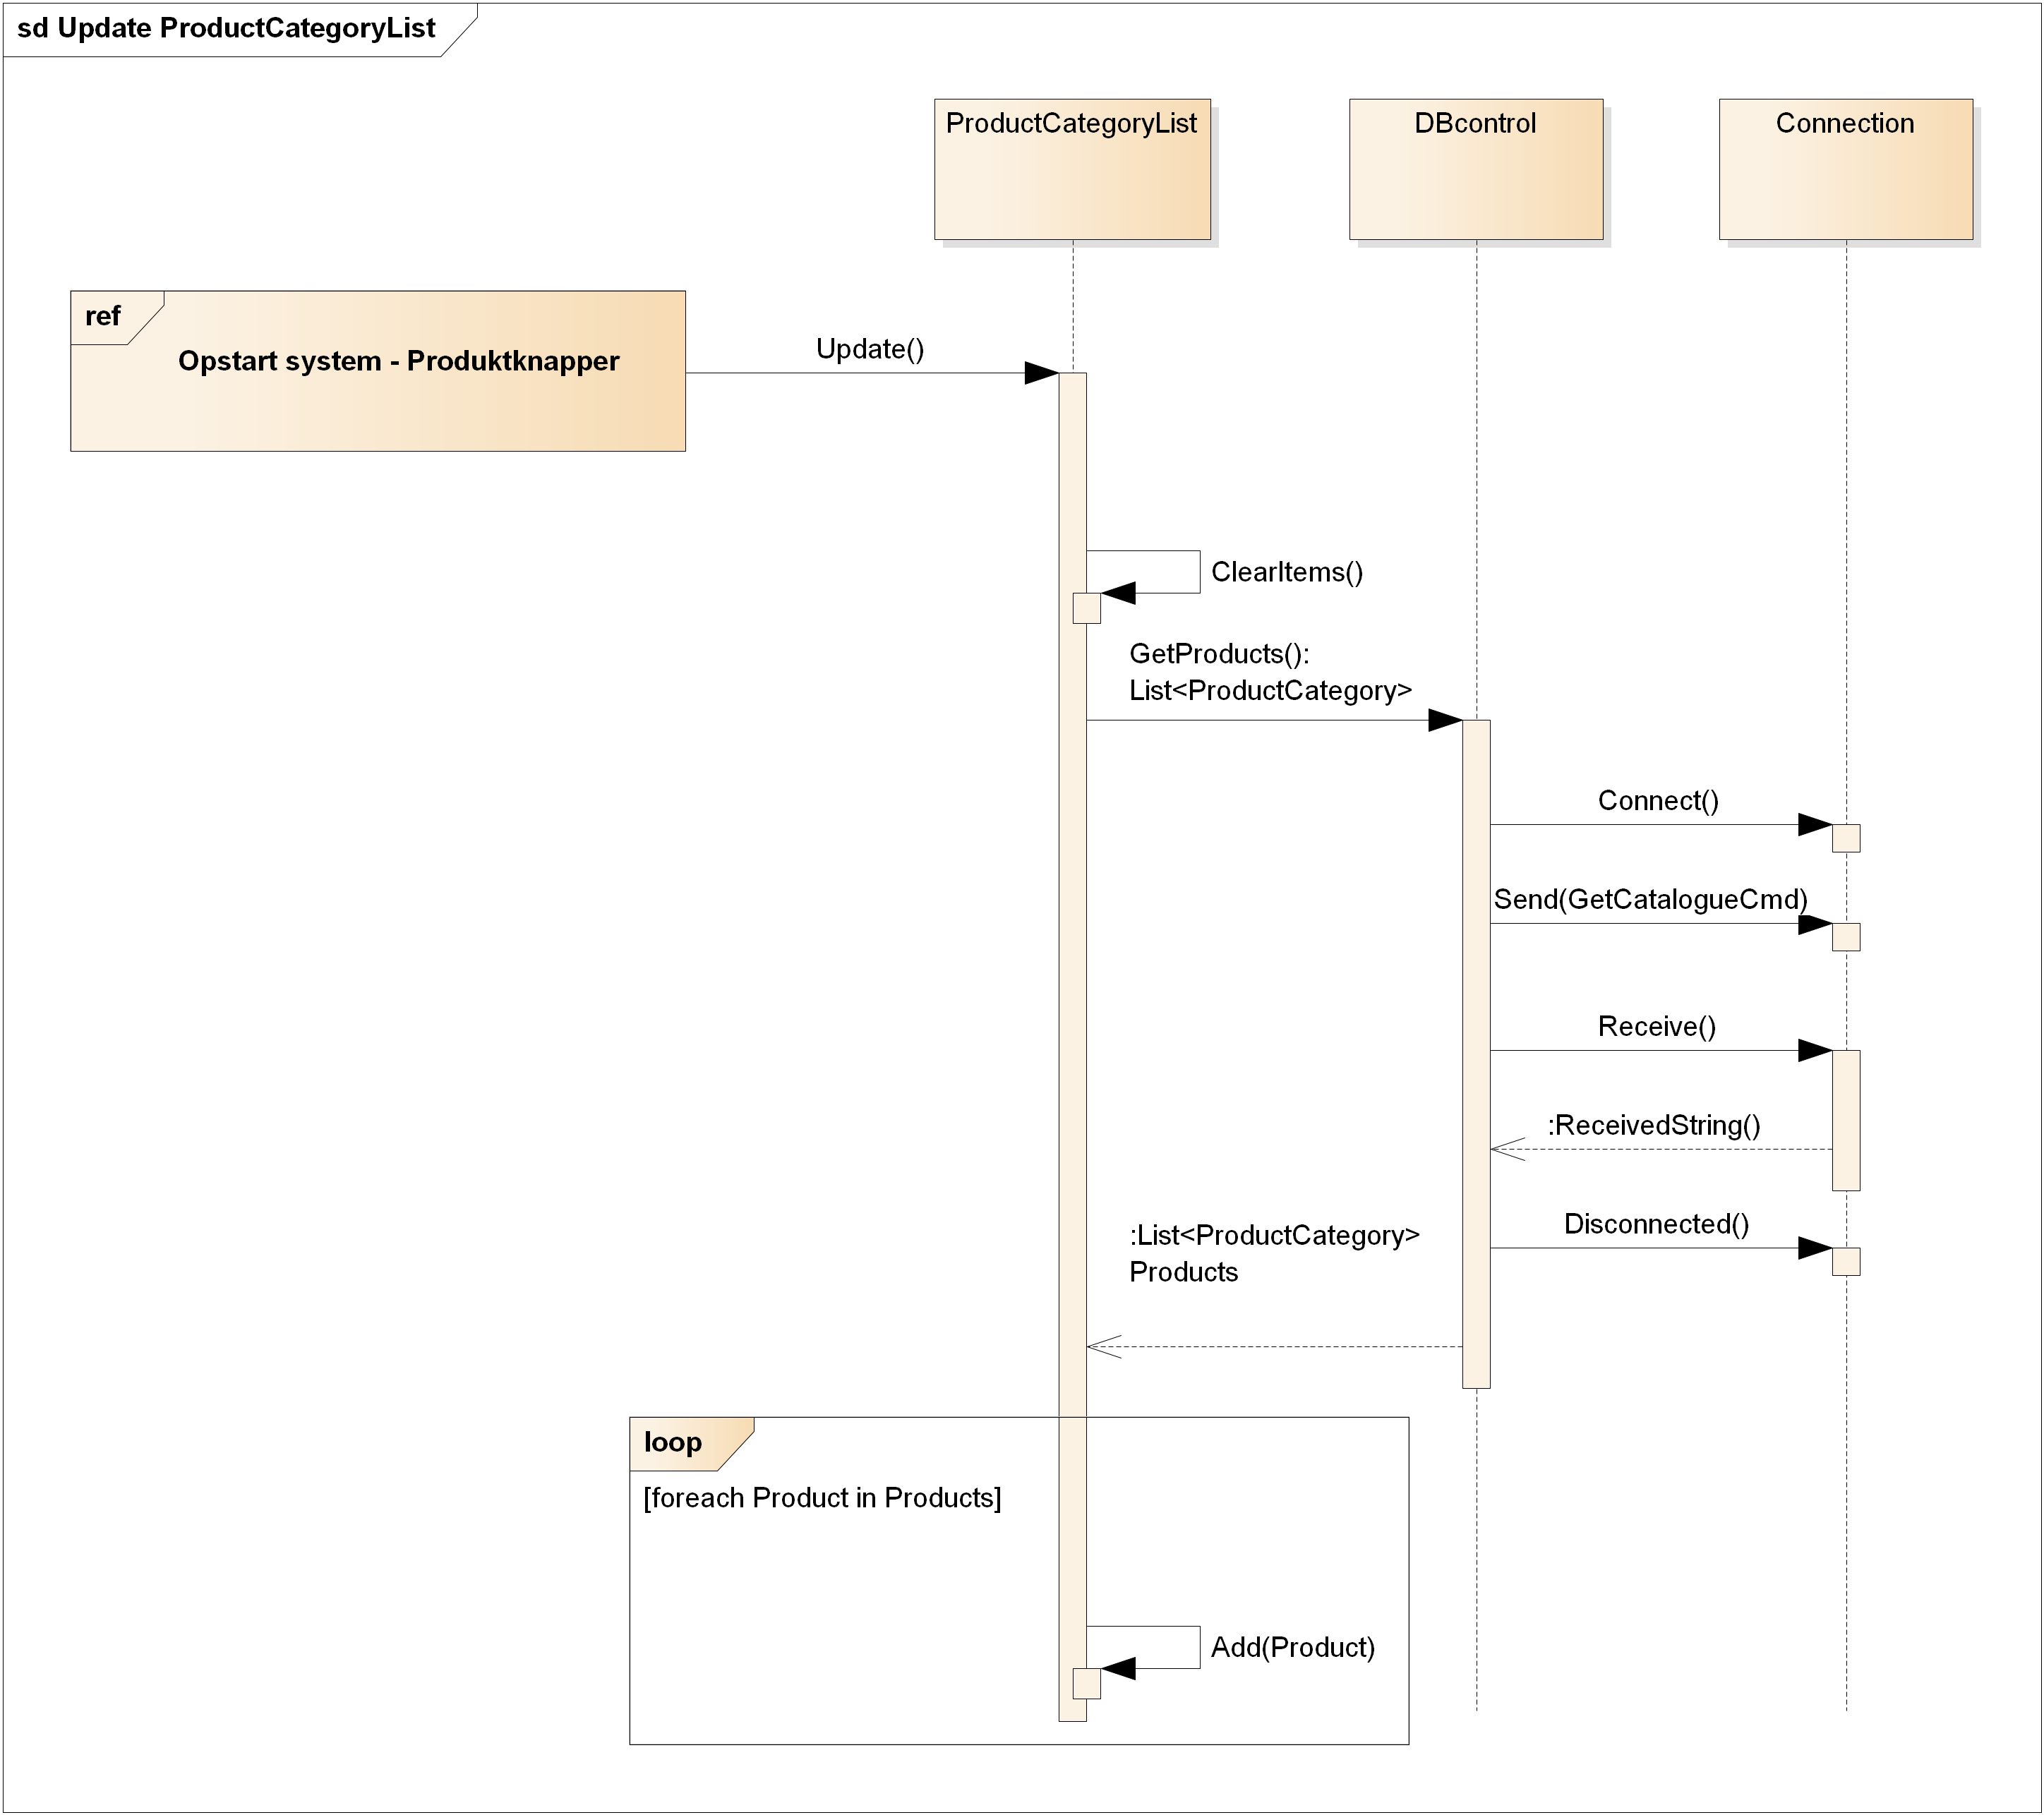
\includegraphics[width=1\textwidth]{Systemdesign/Frontend/GUI/DesignOgStruktur/Pics/UpdateProductCategoryList}
	\caption{Sekvensdiagram over Update ProductCategoryList}
	\label{fig:SekvensUpdatePCL}
\end{figure}

Sekvensdiagrammet på figur \ref{fig:SekvensUpdatePCL} viser hvordan ProductCategoryList bliver opdateret med produkterne i databasen. ProductCategoryList bliver kaldt ved Update, og denne starter så med at kalde \textit{Clear()}. Derefter Kaldes \textit{GetProducts()} i DbControl. Denne klasse opretter så forbindelse til CentralServer ved et kald til Connection og beder herefter om at få tilsendt produktkataloget. Når produktkataloget er modtaget afsluttes forbindelsen og den modtagede data returneres til DbControl. Til sidst tilføjes hver af produkterne fra produktkataloget til ProductCategoryLists interne produktliste.

\begin{figure}[H]
	\centering
	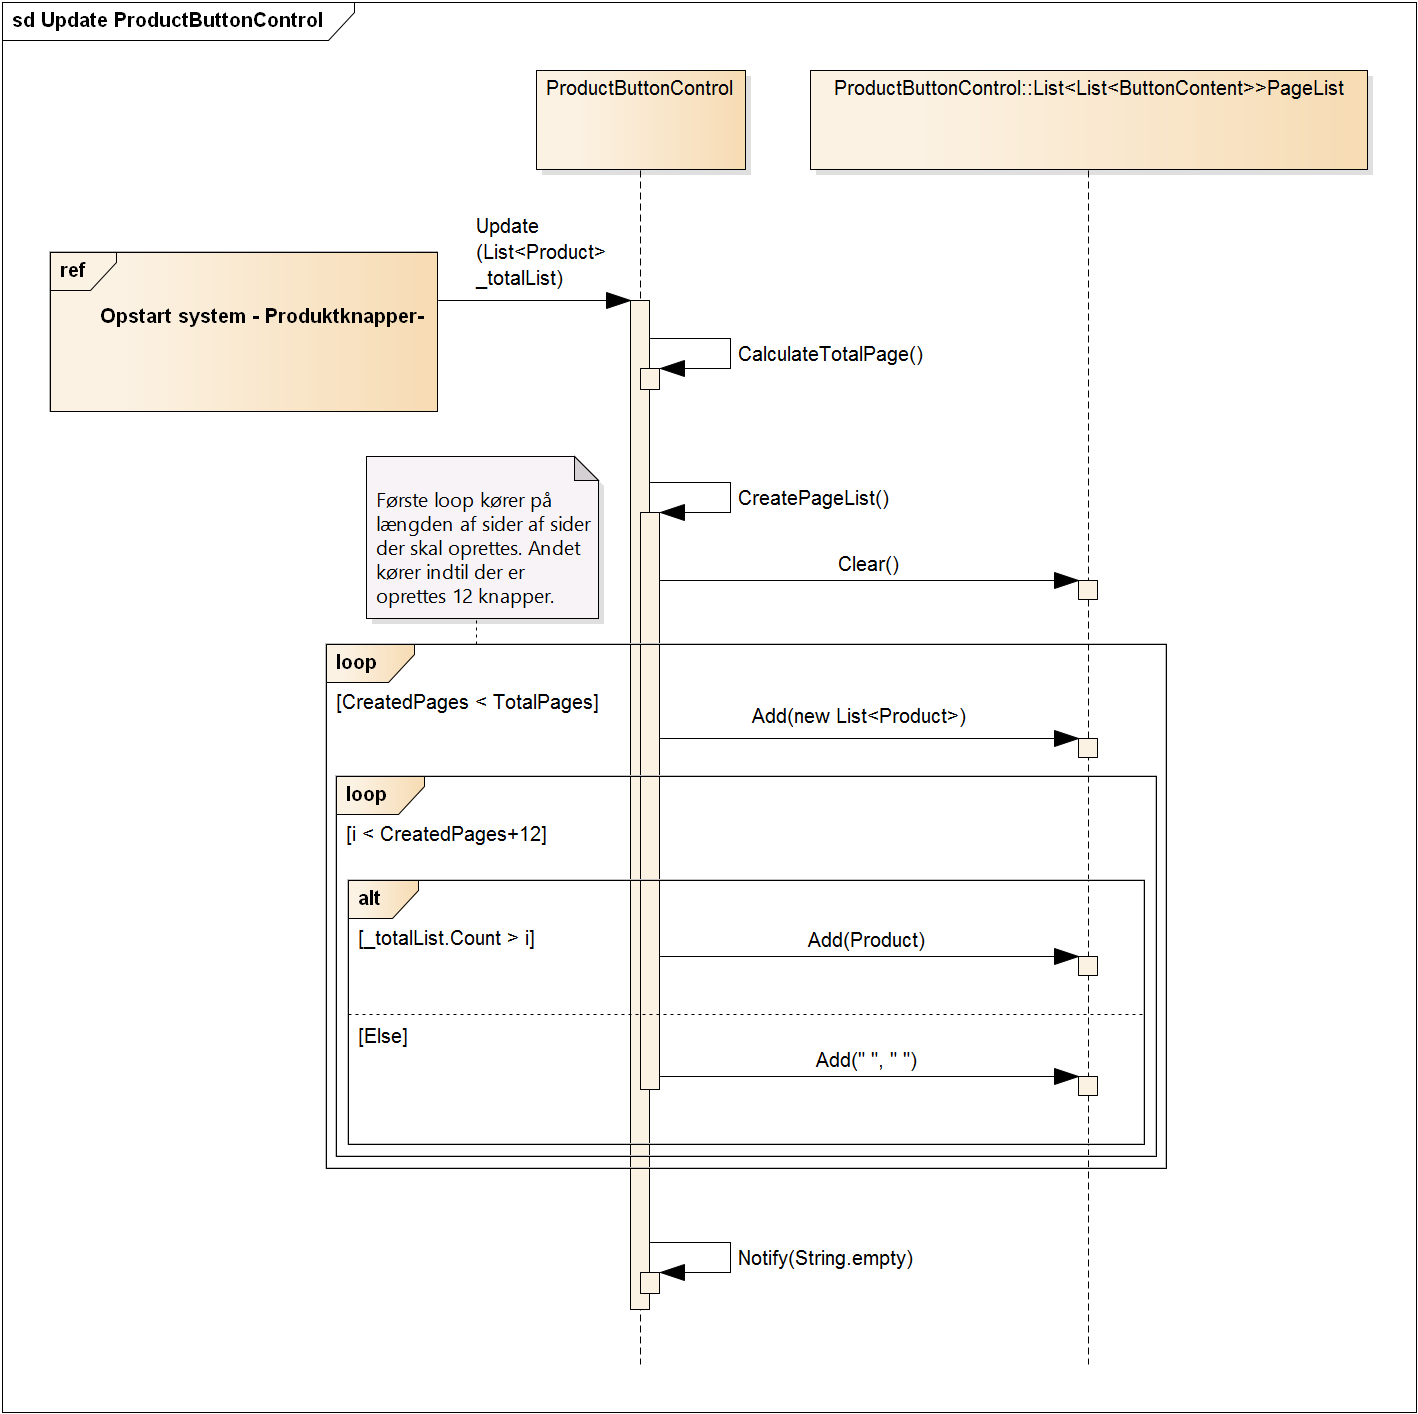
\includegraphics[width=1\textwidth]{Systemdesign/Frontend/GUI/DesignOgStruktur/Pics/UpdateProductButtonControl}
	\caption{Sekvensdiagram over Update ProductButtonControl}
	\label{fig:SekvensUpdatePBC}
\end{figure}

Sekvensdiagrammet på figur \ref{fig:SekvensUpdatePBC} viser hvordan ProductButtonControl opretter PageList som er de sider af produktknapper som kan vises i brugergrænsefladen. ProductButtonControl bliver kaldt ved update med en liste af produkter som parameter. Denne liste bruges så til at udregne den totale mængde af sider ved et kald til metoden \textit{CalculateTotalPage()}. Derefter kaldes \textit{CreatePageList()}. Denne metode starter med at rydde sit indhold, og herefter opretter den en ny liste pr. 12 produkter. Dernæst itererer den over produktlisten og opretter en knap pr. eksisterende produkt.

\newpage
